\documentclass[tikz,border=3pt]{standalone}
\usepackage[utf8]{inputenc}
\usepackage[T1]{fontenc}
\usepackage{lmodern}
\renewcommand{\familydefault}{\sfdefault}
\usepackage{sansmath}\sansmath
\usepackage{chemfig}
\usepackage{pgfplots}\pgfplotsset{compat=1.18,/pgf/number format/use comma,/pgf/number format/1000 sep={.}}
\usetikzlibrary{arrows.meta,calc,positioning,decorations.pathmorphing,patterns}
% paleta del sitio
\definecolor{nar}{HTML}{E8680C}\definecolor{narc}{HTML}{FFB35C}\definecolor{hielo}{HTML}{FFF3E8}
\definecolor{tinta}{HTML}{1D1D1F}\definecolor{gris}{HTML}{6E6E73}\definecolor{lila}{HTML}{7C5CF0}
\definecolor{azul}{HTML}{2F6FD6}\definecolor{menta}{HTML}{17A673}\definecolor{coral}{HTML}{E8342A}
\begin{document}
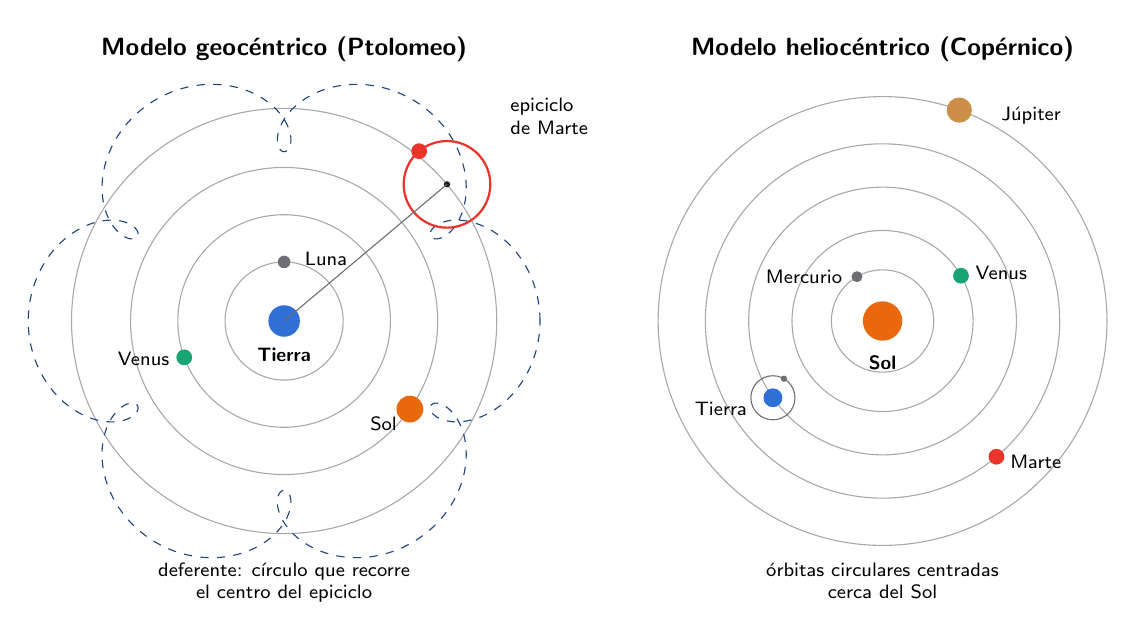
\begin{tikzpicture}[font=\footnotesize,>={Stealth[length=2.2mm]}]
% ---- geocentrico
\begin{scope}
\node[font=\small\bfseries] at (0,3.45) {Modelo geocéntrico (Ptolomeo)};
\foreach \r in {0.75,1.35,1.95,2.7} \draw[gris!60] (0,0) circle (\r);
\draw[azul!60!black,thin,dashed,domain=0:360,samples=400,smooth] plot ({2.7*cos(\x)+0.55*cos(7*\x)},{2.7*sin(\x)+0.55*sin(7*\x)});
\fill[azul] (0,0) circle (0.2); \node[below=3pt,font=\scriptsize\bfseries] at (0,-0.12) {Tierra};
\fill[gris] (90:0.75) circle (0.08); \node[right,font=\scriptsize] at (80:0.8) {Luna};
\fill[menta] (200:1.35) circle (0.1); \node[left,font=\scriptsize] at (200:1.42) {Venus};
\fill[nar] (-35:1.95) circle (0.17); \node[below left,font=\scriptsize] at (-35:1.9) {Sol};
% epiciclo de Marte
\coordinate (C) at (40:2.7);
\draw[coral,thick] (C) circle (0.55); \fill[tinta] (C) circle (0.04);
\fill[coral] ($(C)+(130:0.55)$) circle (0.1);
\draw[gris] (0,0) -- (C);
\node[font=\scriptsize,align=left,anchor=west] at (2.75,2.6) {epiciclo\\de Marte};
\node[font=\scriptsize,align=center,anchor=north] at (0,-2.95) {deferente: círculo que recorre\\el centro del epiciclo};
\end{scope}
% ---- heliocentrico
\begin{scope}[xshift=7.6cm]
\node[font=\small\bfseries] at (0,3.45) {Modelo heliocéntrico (Copérnico)};
\foreach \r in {0.65,1.15,1.7,2.25,2.85} \draw[gris!60] (0,0) circle (\r);
\fill[nar] (0,0) circle (0.25); \node[below=4pt,font=\scriptsize\bfseries] at (0,-0.18) {Sol};
\fill[gris] (120:0.65) circle (0.07); \node[left,font=\scriptsize] at (125:0.68) {Mercurio};
\fill[menta] (30:1.15) circle (0.1); \node[right,font=\scriptsize] at (30:1.22) {Venus};
\fill[azul] (215:1.7) circle (0.12); \node[left,font=\scriptsize] at (215:1.95) {Tierra};
\draw[gris] (215:1.7) circle (0.28); \fill[gris] ($(215:1.7)+(60:0.28)$) circle (0.04);
\fill[coral] (-50:2.25) circle (0.1); \node[right,font=\scriptsize] at (-50:2.33) {Marte};
\fill[narc!80!black] (70:2.85) circle (0.16); \node[right,font=\scriptsize] at (62:2.95) {Júpiter};
\node[font=\scriptsize,align=center,anchor=north] at (0,-2.95) {órbitas circulares centradas\\cerca del Sol};
\end{scope}
\end{tikzpicture}
\end{document}
